\section{Problemas}

\subsection{Estimación de Pose en Humanos}

La tarea de \textit{Estimación de Pose en Humanos} (HPE por sis siglas en inglés) ha sido uno de los
tópicos de gran importancia en
el campo de Visión por Computadora. Debido a la búsqueda de automatización y entendimiento de
diversas actividades humanas, sus utilidades causan impacto directo en las implementaciones
tecnológicas del mundo real, tales como, la predicción de intención (vigilancia), sistemas de
autónomos y de asistencia en la conducción automóviles, animación, simulaciones,
interacción Humano-Computadora (HCI), realidad virtual
aumentada (VR y AR), videojuegos, salud o asistencia médica o hasta análisis de movimiento en
deportes. La tarea de \textit{Estimación de Pose} no solo se limita a el cuerpo
humano, también, puede ser empleado en objetos como carros o animales, vease la imagen \ref{fig:PE-track}.

Con el crecimiento acelerado de \textit{Aprendizaje Profundo} en los últimos años gracias a las
capacidades actuales de potencia de cómputo los métodos basados bajo este enfoque han sobrepasado
a las métodos tradicionales, sin embargo aún existen distintos problemas y retos que siguen presentes
como la oclusión y la ambiguedad de los datos o la dificultad de su obtención para realizar
entrenamientos.

\begin{figure}[ht!]
    \centering
    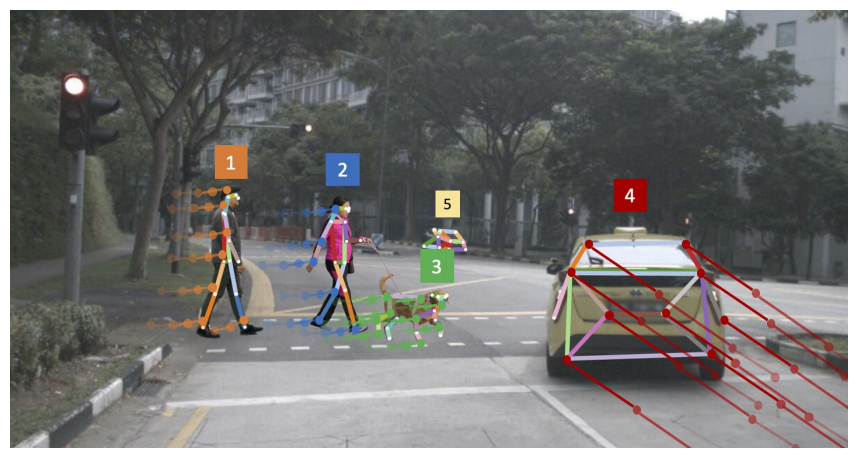
\includegraphics[width=0.4 \textwidth]{Chapters/1. Pose Estimation/figures/openpifpaf.png}
    \caption{OpenPifPaf: Escena del mundo real desde la perspectiva de un carro autónomo. Todos los actores
             son detectados y seguidos, esto incluye a las personas, el carro y el perro. \cite{DBLP:journals/corr/abs-2103-02440}}
    \label{fig:PE-track}
\end{figure}


El problema de \textit{Estimación de Pose Humanos} consiste en predecir las partes del cuerpo o las
posiciones de las articulaciones de una persona a través de una imagen, video. Este problema ha sido
cuidadosamente estudiado a lo largo de los años y diversas recopilaciones de investigaciones han sido escritas.
En la tabla \ref{Tab:hpe-survey} se resumen algunas de las más recientes y que describen dos formas
generales de abordar el problema. La primera de ellas la \quotes{Tradicionalista}, cuyos métodos
usan enfoques clásicos de visión por computadora o la segunda basada en técnicas de aprendizaje
profundo que involucran comúnmente modelos convolucionales. El trabajo realizado en esta tesis está
basado en el segundo método, usando técnicas de aprendizaje profundo y modelos actuales capaces
de capturar información temporal, específicamente enfocado en modelos \textit{Transformers} \cite{Vaswani}.

\begin{table}[ht!]
    \begin{center}
    \resizebox{\textwidth}{!}{%
    \begin{tabular}{|l|l|l|l|}
        % \hline
        % \multicolumn{4}{|c|}{Recopilaciones} \\
        \hline
        \multirow{2}*{\textbf{Título}} & \multirow{2}*{\textbf{Año}} & \textbf{Métodos} & \multirow{2}*{\textbf{Descripción}}\\
         & & \textbf{cubiertos} & \\
        \hline
        \multirow{2}*{A survey of computer vision-based motion capture \cite{MOESLUND2001231}} & \multirow{2}*{2001} & \multirow{2}*{Tradicionales} &  Investigacion general sobre métodos de captura de movimientos basados en visión en\\
        & & & humanos. Incluye estimación de pose, seguimiento y reconocimiento de acciones. \\\hline

        A survey of advances in vision-based human motion capture and analysis \cite{MOESLUND200690} & 2006 & Tradicionales & Incluye una revisión de los métodos de captura de movimiento del año 2001 al 2006.\\ \hline

        \multirow{2}*{Vision-based human motion analysis: An overview. \cite{POPPE20074}} & \multirow{2}*{2007} & \multirow{2}*{Tradicionales} & Investigacion general sobre métodos de captura de movimientos usando datos \\
        & & & sin marcadores de dispositivos de captura. \\\hline

        \multirow{2}*{Advances in view-invariant human motion analysis: A review \cite{5191035}} & \multirow{2}*{2010} & \multirow{2}*{Tradicionales} & Estudio de métodos de estimación de pose en 3D, comportamiento y \\
        & & & reconocimiento/representación de acciones. \\ \hline

        Human pose estimation and activity recognition from multi-view videos: & \multirow{2}*{2012} & \multirow{2}*{Tradicionales} & Métodos de estimación de pose 3D y reconocimiento de acción usando datos \\
        Comparative explorations of recent developments \cite{6193117} &  &  & multi-vista\\ \hline

        A survey of human pose estimation: the body parts parsing based methods \cite{LIU201510} & 2015 & Tradicionales & Estudios de estimación de pose enfocados principalmente a las técnicas de localización \\
        & & & de las distintas partes del cuerpo. \\ \hline

        \multirow{2}*{Human pose estimation from monocular images: A comprehensive survey \cite{Gong2016}} & \multirow{2}*{2016} & \multirow{2}*{Ambos} & Enfocado en la estimación de pose usando datos monoculares incluyendo las\\
        & & & metodologías usadas en procesos tradicionales y basados en aprendizaje profundo. \\ \hline

        \multirow{2}*{3D human pose estimation: A review of the literature and analysis of covariates \cite{SARAFIANOS20161}} & \multirow{2}*{2016} & \multirow{2}*{Deep-Learning} & Revisión general del estado del arte de estimación de pose 3D usando imágenes\\
        & & & y videos RGB. \\ \hline

        \multirow{2}*{Monocular human pose estimation: a survey of deep learning-based methods \cite{CHEN2020102897}} & \multirow{2}*{2020} & \multirow{2}*{Deep-Learning} & Revisión y clasificación general de los métodos de estimación de pose basados en \\
        & & & aprendizaje profundo desde el 2014 usando solo datos monoculares.\\ \hline

        The progress of human pose estimation: a survey and taxonomy \cite{9144178} & \multirow{2}*{2020} & \multirow{2}*{Deep-Learning} & Revisión de los métodos basados en aprendizaje profundo para estimación de \\
        of models applied in 2D human pose estimation &  & & pose 2D\\ \hline

        Deep Learning-Based Human Pose Estimation: A Survey \cite{DBLP:journals/corr/abs-2012-13392} & 2020 & Deep-Learning & Estudio general del estado del arte de estimación de pose 2D y 3D.\\ \hline
    \end{tabular}}
    \end{center}
    \caption{Listado de diversas investigaciones de \textit{Estimación de Pose en Humanos} que abarcan
             tanto enfoques tradicionales como basados en aprendizaje profundo.
             Tabla basada en el trabajo de \citeauthor*{DBLP:journals/corr/abs-2012-13392}.}
    \label{Tab:hpe-survey}
\end{table}

\subsubsection{Taxonomía de Estimación de Pose 2D y 3D}


\begin{figure}\begin{center}
\begin{tikzpicture}[node distance=1.5cm,
        every node/.style={fill=white, font=\sffamily, scale=0.7}, align=center,
        >={Latex[width=2mm,length=2mm]},
        % Specifications for style of nodes:
        % base/.style = {rectangle, rounded corners, draw=black,
        %                 minimum width=4cm, minimum height=1cm,
        %                 text centered, font=\sffamily},
        % activityStarts/.style = {base, fill=blue!30},
        % startStop/.style = {base, fill=red!30},
        % activityRuns/.style = {base, fill=green!30},
        % process/.style = {base, minimum width=2.5cm, fill=blue!10, font=\ttfamily}
        ]
    % Specification of nodes (position, etc.)
    \node (HPE)          []              {HPE};
    \node (2D HPE)       [below of=HPE, left=7.5em of HPE]          {2D HPE};
    \node (3D HPE)       [below of=HPE, right=7.5em of HPE]   {3D HPE};

    \node (2D Single)    [below of= 2D HPE, left=1.0em of 2D HPE]          {2D Single};
    \node (2D Multiple)  [below of= 2D HPE, right=1.0em of 2D HPE]   {2D Multiple};

    \node (3D Single)    [below of= 3D HPE, left=1.0em of 3D HPE]          {3D Single \\ Mono/Multi-view};
    \node (3D Multiple)  [below of= 3D HPE, right=1.0em of 3D HPE]   {3D Multiple};

    \node (2D-Regresion) [below of= 2D Single, left=-1.5em of 2D Single]   {Regresion};
    \node (2D BPD)       [below of= 2D Single, right=-1.5em of 2D Single]   {Body Part \\ Detection};

    \node (2D-TD)        [below of= 2D Multiple, left=-1.5em of 2D Multiple]   {Top-Down};
    \node (2D-BU)        [below of= 2D Multiple, right=-1.5em of 2D Multiple]   {Bottom-Up};

    \node (3D-MF)        [below of= 3D Single, left=-1.5em of 3D Single]   {Model-Free};
    \node (3D-MB)        [below of= 3D Single, right=-1.5em of 3D Single]   {Model-Based};

    \node (3D-TD)        [below of= 3D Multiple, left=-1.5em of 3D Multiple]   {Top-Down};
    \node (3D-BU)        [below of= 3D Multiple, right=-1.5em of 3D Multiple]   {Bottom-Up};

    % \node (onResumeBlock)     [process, below of=onStartBlock]   {onResume()};
    % \node (activityRuns)      [activityRuns, below of=onResumeBlock]
    %                                                     {Activity is running};
    % \node (onPauseBlock)      [process, below of=activityRuns, yshift=-1cm]
    %                                                             {onPause()};
    % \node (onStopBlock)       [process, below of=onPauseBlock, yshift=-1cm]
    %                                                                 {onStop()};
    % \node (onDestroyBlock)    [process, below of=onStopBlock, yshift=-1cm]
    %                                                             {onDestroy()};
    % \node (onRestartBlock)    [process, right of=onStartBlock, xshift=4cm]
    %                                                             {onRestart()};
    % \node (ActivityEnds)      [startStop, left of=activityRuns, xshift=-4cm]
    %                                                     {Process is killed};
    % \node (ActivityDestroyed) [startStop, below of=onDestroyBlock]
    %                                                 {Activity is shut down};
    % Specification of lines between nodes specified above
    % with additional nodes for description
    \draw[-]             (HPE) -- (2D HPE);
    \draw[-]             (HPE) -- (3D HPE);
    \draw[-]             (2D HPE) -- (2D Single);
    \draw[-]             (2D HPE) -- (2D Multiple);
    \draw[-]             (3D HPE) -- (3D Single);
    \draw[-]             (3D HPE) -- (3D Multiple);
    \draw[-]             (2D Single) -- (2D-Regresion);
    \draw[-]             (2D Single) -- (2D BPD);
    \draw[-]             (2D Multiple) -- (2D-TD);
    \draw[-]             (2D Multiple) -- (2D-BU);
    \draw[-]             (3D Single) -- (3D-MF);
    \draw[-]             (3D Single) -- (3D-MB);
    \draw[-]             (3D Multiple) -- (3D-TD);
    \draw[-]             (3D Multiple) -- (3D-BU);

    % \draw[->]      (onStartBlock) -- (onResumeBlock);
    % \draw[->]     (onResumeBlock) -- (activityRuns);
    % \draw[->]      (activityRuns) -- node[text width=4cm]
    %                                 {Another activity comes in
    %                                 front of the activity} (onPauseBlock);
    % \draw[->]      (onPauseBlock) -- node {The activity is no longer visible}
    %                                 (onStopBlock);
    % \draw[->]       (onStopBlock) -- node {The activity is shut down by
    %                                 user or system} (onDestroyBlock);
    % \draw[->]    (onRestartBlock) -- (onStartBlock);
    % \draw[->]       (onStopBlock) -| node[yshift=1.25cm, text width=3cm]
    %                                 {The activity comes to the foreground}
    %                                 (onRestartBlock);
    % \draw[->]    (onDestroyBlock) -- (ActivityDestroyed);
    % \draw[->]      (onPauseBlock) -| node(priorityXMemory)
    %                                 {higher priority $\rightarrow$ more memory}
    %                                 (ActivityEnds);
    % \draw           (onStopBlock) -| (priorityXMemory);
    % \draw[->]     (ActivityEnds)  |- node [yshift=-2cm, text width=3.1cm]
    %                                 {User navigates back to the activity}
    %                                 (onCreateBlock);
    % \draw[->] (onPauseBlock.east) -- ++(2.6,0) -- ++(0,2) -- ++(0,2) --
    %     node[xshift=1.2cm,yshift=-1.5cm, text width=2.5cm]
    %     {The activity comes to the foreground}(onResumeBlock.east);
\end{tikzpicture}
\caption{M1 caption for diagram} \label{fig:HPE-diagram}
\end{center} \end{figure}

\textbf{Estimación de Pose en 2 y 3 dimensiones}

Existen dos grandes grupos que dividen las metodologías seguidas para la \textit{Estimación de Pose en
Humanos}; estimación de pose en 2 y 3 dimensiones. Cómo el nombre lo sugiere, la \textit{Estimación
de Pose 2D} (\textbf{2D HPE} por sus siglas en inglés) consiste en localizar articulaciones o partes del cuerpo
directamente en imágenes, por tanto, el marco de referencia de las posiciones de cada articulación es la
propia imagen. En la \textit{Estimación de Pose 3D} (\textbf{3D HPE}) las elementos detectados pasan a estar en 3D
y se busca un marco de referencia que mejor se ajuste las dimensiones espaciales de las
articulaciones y personas. Comúnmente se usa un cubo unitario cuyo centro corresponde a la
articulación que indica la cadera o \textit{hip} como se encuentra en la literatura, véase la figura
\ref{fig:HPE-diagram}.

Por otro lado, en muchos escenarios las imágenes contienen más de una persona o se necesita hacer seguimiento
de multiples individuos. Por lo regular cuando aparecen más de un persona en una imagen
(\textbf{MPPE}, Multiple Person Pose Estimation)
se opta por identificar cada cuerpo en la imagen y posteriormente resolver individualmente
la estimación de pose para cada una de las entidades identificadas (\textbf{SPPE}, Single Pose Estimation).
La detección de los cuerpos se realiza en
etapas previas usando modelos de detección de objetos y entrenados para detectar cuerpos
humanos tales como \textit{MobileNet} \cite{DBLP:journals/corr/RenHG015}
\cite{DBLP:journals/corr/HowardZCKWWAA17} \cite{DBLP:journals/corr/abs-1801-04381} o \textit{YOLO}
(You Only Look Once) \cite{DBLP:journals/corr/RedmonDGF15} \cite{DBLP:journals/corr/abs-2004-10934}.

Además, el proceso de estimación de pose puede ser realizado en multiples etapas. Es decir, un modelo
end-to-end puede realizar la tarea completamente o en caso contrario, dividir la tarea en multiples
etapas y usar modelos especializados para resolver cada etapa. Por ejemplo en estimación de pose 3D
es común predecir la pose 2 dimensiones usando una red entrenada para esta tarea y posteriormente
pasar a 3 dimensiones usando la información previa \cite{DBLP:journals/corr/MartinezHRL17}.

\textbf{Estimación de Pose 2D Single}.
Para la estimación de pose en 2D dónde solo es involucrada una sola personas se usan dos enfoques,
los métodos basado en regresión (\textit{Regresion-Based}) y los métodos basados en detección de
partes del cuerpo humano ((\textit{Detection-Based o Body Part Detection})). Los métodos basados en
regresión estiman las posiciones relacionando directamente la imagen con las coordenadas de las
articulaciones del modelo de cuerpo humano usado. En cambio, los métodos basados de detección
identifican primeramente las partes del cuerpo ya sea a través de marcas como recuadros de las
posiciones o usando mapas de calor que indican las posiciones de las articulaciones.

\textbf{Estimación de Pose 3D Single}.
Existen dos métodos generales para la estimación de pose 3D en una sola personas, los
\textit{Generativos} y los \textit{Discriminativos}. Los métodos Generativos
también conocidos como (\textit{model-based}, basado en modelos) usan alguna representación de modelos
del cuerpo humano en conjunto con información apriori como los movimientos y el contexto en el que se
ejecutan. Las poses son predecidas usando la imágen un conjunto de representaciones obtenidos de establecer un
función de probabilidad usando información tal como descriptores de la imagen, la estructura del cuerpo
humano, los parámetros de las cámaras y y un conjunto de restricciones derivadas del contexto. Los
modelos Discriminativos simplemente aprenden a predecir directamente la pose usando la datos de entrada
sin usar información de modelos humanos.

\textbf{Estimación de Pose 2D-3D Multiple}.

% Mono  https://sci-hub.se/10.1109/access.2020.3010248 26-30
% Multi https://sci-hub.se/10.1109/access.2020.3010248 31-35

Top-Down El procesamiento se realiza primero detectando los personas individualmente en la imagen
usando un bounding-box proporcionado por algun detector de objetos. [26, 27, 29].
EL principal problema de este enfoque es que si la detección de la persona falla ya no hay nada más
que hacer, y el costo computacional depende de la cantidad de personas en la imagen, puesto que para
cada persona detectada es necesario correr un estimador de pose entrenado para detectar una sola
persona.

Bottom-Up: [31, 34] En este enfoque se inicia localizando entidades semánticas y luego agrupandolas
para formar una persona. Claramente usando este procedimiento el problema de rendimiento de usar un
estimador de pose por cada persona desaparece, pues todas las entidades de los cuerpos son detectados
a la vez y posteriormente agrupados para formar cada persona. Sin embargo, el modelo generado tiende
a presentar problemas cuando existen personas ocluyéndose unas a otras.


La estimación de pose en 3d también puede ser realizado en dos dos marcos, \textit{monocular}
cuando solo se tiene una imagen de reference del sujeto de prueba en un tiempo o pose exacta y
multi-vista cuando se tienen imágenes desde diferentes perspectivas del sujeto de prueba en misma
la pose y tiempo exacto. La ventaja de usar técnicas que puedan aprovechar la información contenida
en diferentes perspectivas es que ayuda a reducir en gran medida la ambigüedad ocasionada por las
oclusiones, una parte puede no ser visible desde un ángulo pero desde otro si. Sin embargo, la
cantidad de conjunto de datos existentes para estimación de pose multi-vista es reducida.


Largely three kinds of loss functions applied in human pose estimation models, namely, Mean Absolute
Error (MAE), Mean Squared Error (MSE), and Cross-Entropy loss


\textbf{Tipos de datos}.

En los últimos años, debido a la masificación
de dispositivos inteligentes, el acceso a una cámara digital no resulta un problema mayor para la muchas
de las personas, así, la mayoría de los trabajos realizados sobre Estimación de Pose usan
\textit{Imágenes RGB} gracias a su fácil captura y acceso.
Sin embargo, esto solo es cierto en el contexto de la Estimación de Pose 2D, puesto que el etiquetado de datos
usando las coordenadas de la imagen como referencia no representa demasiado problema. En la
Estimación de Pose 3D, la complejidad de la obtención de los datos se incrementa. Para llevar a cabo
el proceso de obtención de los datos es necesario usar equipo especializado y costoso para la captura
de movimiento en acompañamiento de las cámaras de video \cite{6682899}. Hay dos mecanismos de captura
de movimiento, los ópticos y los no ópticos. Generalmente, en los primeros el sujeto de prueba no
necesita de aditamentos complejos como el uso de trajes
(exoesqueleto) y solo un software con ayuda de cámaras, sensores y marcadores se
encargan de registrar e interpretar el movimiento a un modelo digital. Si bien
aventajan en una reducción de coste su precisión es menor que los no ópticos.
El \textit{Kinect}, fabricado por \textit{Microsoft} es uno de los dispositivos más usados
para generar imágenes de infrarrojos (\textit{IR-image}) siendo de fácil encontrarlo y adquirirlo
gracias a su bajo conste. \cite{6165146} \cite{Izadi11kinectfusion:real-time}.

Por otra parte, existen dispositivos basados en tecnologías como \textit{LIDAR} cuya función es
generar imágenes de profundad. Al igual que el \textit{Kinect}, cada vez son de más fácil acceso
debido a su comercialización en dispositivos inteligentes en el último año por compañías como Apple
\cite{DBLP:journals/corr/abs-1711-06396}. El segundo tipo se puede dividir en dos clases;
los mecánicos los cuales usan giroscopios y acelerómetros para registrar el
movimiento y los electromagnéticos, cuyo funcionamiento es a través de la generación un campo
electromagnético y para posteriormente capturar las alteraciones en este que realiza el sujeto al
moverse \cite{articleMotion}.


\textbf{Modelación del Cuerpo Humano}

Skeleton base model or stick figure or kinematic model
Es uno de los modelos más simples y mayormente usados. Consiste en grafo de nodos que representan
las articulaciones del cuerpo humano, comúnmente entre 10 y 30 nodos \cite{Felzenszwalb2005}.
Así, un hueso es representado como una conexión entre dos articulaciones. Al ser solo una
representación de la estructura del cuerpo carece de demás información como texturas o formas.

Contour base model or Planar Model
Es uno de los primeros modelos usados para problemas de Estimación de Pose. Los miembros y torso del
cuerpo humano son representados como un conjunto de rectángulos que proveen información tanto de los
límites de cada miembros como sus longitudes y anchor \cite{557241} \cite{COOTES199538}

Volumen base model
Es usado para representar el cuerpo humano y su volumen, es decir es una representación 3D del
cuerpo conseguida a través de un mallado de figuras geométricas y capturados por escaner 3D
\cite{840661}.


\textbf{Conjuntos de Datos más usados}

MPII: The MPII human pose dataset is a multi-person 2D Pose Estimation dataset comprising of nearly
500 different human activities, collected from Youtube videos. MPII was the first dataset to contain
such a diverse range of poses and the first dataset to launch a 2D Pose estimation challenge in 2014

COCO: The COCO keypoints dataset is a multi-person 2D Pose Estimation dataset with images collected
from Flickr. COCO is the largest 2D Pose Estimation dataset, to date, and is considering a benchmark
for testing 2D Pose Estimation algorithms.

HumanEva : HumanEva is a single-person 3D Pose Estimation dataset, containing video sequences
recorded using multiple RGB and grayscale cameras. Ground truth 3D poses are captured using
marker-based motion capture (mocap) cameras. HumanEva was the first 3D Pose Estimation dataset of
substantial size.

Human3.6M : Human3.6M is a single-person 2D/3D Pose Estimation dataset, containing video sequences
in which 11 actors are performing 15 different possible activities were recorded using RGB and
time-of-flight (depth) cameras. 3D poses are obtained using 10 mocap cameras. Human3.6M is the
biggest real 3D Pose Estimation dataset, to date.

SURREAL : SURREAL is a single-person 2D/3D Pose Estimation dataset, containing virtual video
animations created using mocap data recorded in the lab. SURREAL is the biggest 3D Pose Estimation
dataset, but is not yet accepted as a benchmark for comparing 3D Pose Estimation algorithms. This
is mainly because it is a synthetic dataset.

Modern pose estimation algorithms are almost exclusively based on convolutional neural networks
with hourglass architecture or its variants (see the image below). Such a network consists of two
major parts: a convolutional encoder that compresses the input image into the so-called latent
representation and decoder that constructs N heatmaps from the latent representation where N is the
number of searched keypoints.

Why is it hard?
Strong articulations, small and barely visible joints, occlusions, clothing, and lighting changes
make this a difficult problem.
Main challenges -> https://viso.ai/deep-learning/pose-estimation-ultimate-overview/

The major challenges for tracking poses from the car perspective are
(i) occlusions due to the viewing angle and (ii) prediction
speed to be able to react to real-time changes in the environ

Biased databases
La mayoría de la bases de datos son obtenidas a través de algunos pocos sujetos de prueba.
La estructura fisiológica de individuos no es perfecta y pueden variar debido a diversos factores
como el sexo, la raza, edad, lugar de nacimiento y desarrollo, enfermedades, factores genéticos, entre
otros, además de que los movimientos recreados entre sujetos no siempre son hechos de la misma manera
aunque las circunstancias o ambiente esté controlado.

Irregularidades en los datos reales.
Si los datos son obtenidos bajo un ambiente controlado es posible obtener imágenes fieles para el
entrenamiento. Por otro lodo, los modelos al ser desplegados y puestos en marcha en ambientes reales
se enfrentan a imprevistos de los que no se puede tener control; oclusiones de diversas partes del
cuerpo ya sea por el mismo sujeto o algún objeto extraño en la captura, movimientos extraños o rápidos
como correr o dar una patada donde el modelo no puede los puede identificar o el equipo de captura
no pueda obtener que se ven como fotogramas borrosos.

Monocular human pose estimation has some unique characteristics
and challenges:

Flexible body configuration indicates complex interdependent
joints and high degree-of-freedom limbs, which may cause self occlusions or rare/complex poses.
- Diverse body appearance includes different clothing and self similar parts.
- Complex environment may cause foreground occlusion, occlusion
or similar parts from nearby persons, various viewing angles, and
truncation in the camera view


\subsubsection{Métricas de Evaluación}

% Percentage of Correct Parts (PCP): this metric measures
% the detection rate of limbs. A limb (body part) is considered
% detected if the distance between the two predicted joint
% locations and the true limb joint locations is less than half of
% the limb length [46]. PCP commonly referred also as
% PCP-0.5. Recently, PCP has not been preferred as an
% evaluation metric even though it was initially regarded as the
% go-to metric. This is because PCP penalizes shorter limbs. The
% higher the PCP the better the model.

% Percentage of Detected Joints(PDJ): this metric is proposed
% to address the limitations observed in PCP. This evaluation
% metric defines a joint correctly detected if the distance
% between the predicted joint location and the true joint location
% is within a certain fraction of the torso diameter (the distance
% between the right hip and left shoulder). For instance, for
% PDJ-0.2, it means the distance between the predicted joint
% location and the true joint location should be less than 0.2 *
% torso diameter. By changing this fraction, detection rates are
% obtained for different degrees of localization precision


% Percentage of Correct Key-points(PCK): this also measures
% the distance between the predicted joint location and the true
% joint location. The PCK evaluation metric measures the body
% joints’ localization accuracy. The criteria of PCK and PDJ are
% very similar except to the fact that the torso diameter is
% replaced with the maximum side length (or threshold) of the
% external rectangle of ground truth body joints [62]. Thus,
% detecting a joint is considered correct if the distance between
% the predicted joint and the true joint is within a certain fraction
% of the specified threshold. Again, the higher the PCK the better
% the model

% PCKh is a modified version of PCK. PCKhs matching
% threshold is 50% of the head segment length (a portion of the
% head length is used as a reference at 50%). PCKh is also
% defined as the head-normalized probability of the correct
% keypoint metric [63]. In PCKh, joint detection is considered
% correct if the predicted joint location is with a certain threshold
% from the true joint location. But the threshold should be
% adaptively selected based on the individual’s size. It should
% fall within αl pixels of the ground-truth position, where α is a
% constant and l is the head size that corresponds to 60% of the
% diagonal length of the ground-truth head bounding box. The
% PCKh@0.5 (α = 0.5) score is reported [63]. To make the
% metric articulation independent, one probably better chooses
% to use the head size.


% Area Under the Curve (AUC) measures the different range
% PCK thresholds (E.g., when α varies from 0 to 0.5) entirely. It
% informs how the model is capable of distinguishing each
% body's joints. The higher the AUC, the better the model


% Area Under the Curve (AUC) measures the different range
% PCK thresholds (E.g., when α varies from 0 to 0.5) entirely. It
% informs how the model is capable of distinguishing each
% body's joints. The higher the AUC, the better the model

% Object Keypoint Similarity (OKS) gives a measure of how
% a predicted keypoint is close to ground truth. OKS is much
% similar to IoU (Intersection over Union) in keypoint detection
% performance. So, when a model gets higher OKS, it means the
% overlap between the predicted keypoint and the truth is higher.

% Besidesthe above evaluation metrics, Average Precision (AP)
% and mean Average Precision (mAP) are also used [64, 65]

\subsection{Lung Pathologies detection}
